\setcounter{enumi}{0}
\makeatletter
\renewcommand{\theenumi}{\@Roman\c@enumi}
\makeatother
%
\begin{table}[htbp]
\makebox[0pt][l]{\begin{tabular}{lll|lll}
\hline
 名前 & 表示 & CMYK値 &  名前 & 表示 & CMYK値 \\
\hline
\cc{GreenYellow}   {0.15, 0, 0.69, 0} &
\cc{RoyalPurple}   {0.75, 0.90, 0, 0} \\
\cc{Yellow}        {0, 0, 1, 0}       &
\cc{BlueViolet}    {0.86, 0.91, 0, 0.04} \\
\cc{Goldenrod}     {0, 0.10, 0.84, 0} &
\cc{Periwinkle}    {0.57, 0.55, 0, 0}\\
\cc{Dandelion}     {0, 0.29, 0.84, 0} &
\cc{CadetBlue}     {0.62, 0.57, 0.23, 0}\\
\cc{Apricot}       {0, 0.32, 0.52, 0} &
\cc{CornflowerBlue}{0.65, 0.13, 0, 0}\\
\cc{Peach}         {0, 0.50, 0.70, 0} &
\cc{MidnightBlue}  {0.98, 0.13, 0, 0.43}\\
\cc{Melon}         {0, 0.46, 0.50, 0} &
\cc{NavyBlue}      {0.94, 0.54, 0, 0}\\
\cc{YellowOrange}  {0, 0.42, 1, 0}    &
\cc{RoyalBlue}     {1, 0.50, 0, 0}\\
\cc{Orange}        {0, 0.61, 0.87, 0} &
\cc{Blue}          {1, 1, 0, 0}\\
\cc{BurntOrange}   {0, 0.51, 1, 0}    &
\cc{Cerulean}      {0.94, 0.11, 0, 0}\\
\cc{Bittersweet}   {0, 0.75, 1, 0.24} &
\cc{Cyan}          {1, 0, 0, 0}\\
\cc{RedOrange}     {0, 0.77, 0.87, 0} &
\cc{ProcessBlue}   {0.96, 0, 0, 0}\\
\cc{Mahogany}      {0, 0.85, 0.87, 0.35}&
\cc{SkyBlue}       {0.62, 0, 0.12, 0}\\
\cc{Maroon}        {0, 0.87, 0.68, 0.32}&
\cc{Turquoise}     {0.85, 0, 0.20, 0}\\
\cc{BrickRed}      {0, 0.89, 0.94, 0.28}&
\cc{TealBlue}      {0.86, 0, 0.34, 0.02}\\
\cc{Red}           {0, 1, 1, 0}       &
\cc{Aquamarine}    {0.82, 0, 0.30, 0}\\
\cc{OrangeRed}     {0, 1, 0.50, 0}    &
\cc{BlueGreen}     {0.85, 0, 0.33, 0}\\
\cc{RubineRed}     {0, 1, 0.13, 0}    &
\cc{Emerald}       {1, 0, 0.50, 0}\\
\cc{WildStrawberry}{0, 0.96, 0.39, 0} &
\cc{JungleGreen}   {0.99, 0, 0.52, 0}\\
\cc{Salmon}        {0, 0.53, 0.38, 0} &
\cc{SeaGreen}      {0.69, 0, 0.50, 0}\\
\cc{CarnationPink} {0, 0.63, 0, 0}    &
\cc{Green}         {1, 0, 1, 0}\\
\cc{Magenta}       {0, 1, 0, 0}       &
\cc{ForestGreen}   {0.91, 0, 0.88, 0.12}\\
\cc{VioletRed}     {0, 0.81, 0, 0}    &
\cc{PineGreen}     {0.92, 0, 0.59, 0.25}\\
\cc{Rhodamine}     {0, 0.82, 0, 0}    &
\cc{LimeGreen}     {0.50, 0, 1, 0}\\
\cc{Mulberry}      {0.34, 0.90, 0, 0.02}&
\cc{YellowGreen}   {0.44, 0, 0.74, 0}\\
\cc{RedViolet}     {0.07, 0.90, 0, 0.34}&
\cc{SpringGreen}   {0.26, 0, 0.76, 0}\\
\cc{Fuchsia}       {0.47, 0.91, 0, 0.08}&
\cc{OliveGreen}    {0.64, 0, 0.95, 0.40}\\
\cc{Lavender}      {0, 0.48, 0, 0} &
\cc{RawSienna}     {0, 0.72, 1, 0.45}\\
\cc{Thistle}       {0.12, 0.59, 0, 0} &
\cc{Sepia}         {0, 0.83, 1, 0.70}\\
\cc{Orchid}        {0.32, 0.64, 0, 0} &
\cc{Brown}         {0, 0.81, 1, 0.60}\\
\cc{DarkOrchid}    {0.40, 0.80, 0.20, 0} &
\cc{Tan}           {0.14, 0.42, 0.56, 0}\\
\cc{Purple}        {0.45, 0.86, 0, 0} &
\cc{Gray}          {0, 0, 0, 0.50}\\
\cc{Plum}          {0.50, 1, 0, 0} &
\cc{Black}         {0, 0, 0, 1}\\
\cc{Violet}        {0.79, 0.88, 0, 0} &
\cc{White}         {0, 0, 0, 0}\\
\hline
\end{tabular}}
\begin{center}
\kuti{\textsf{color}パッケージで標準的に使用できる色の名前\label{kuti:color}}
\end{center}
\end{table}

\clearpage
%
\begin{figure}[htbp]
\begin{center}
   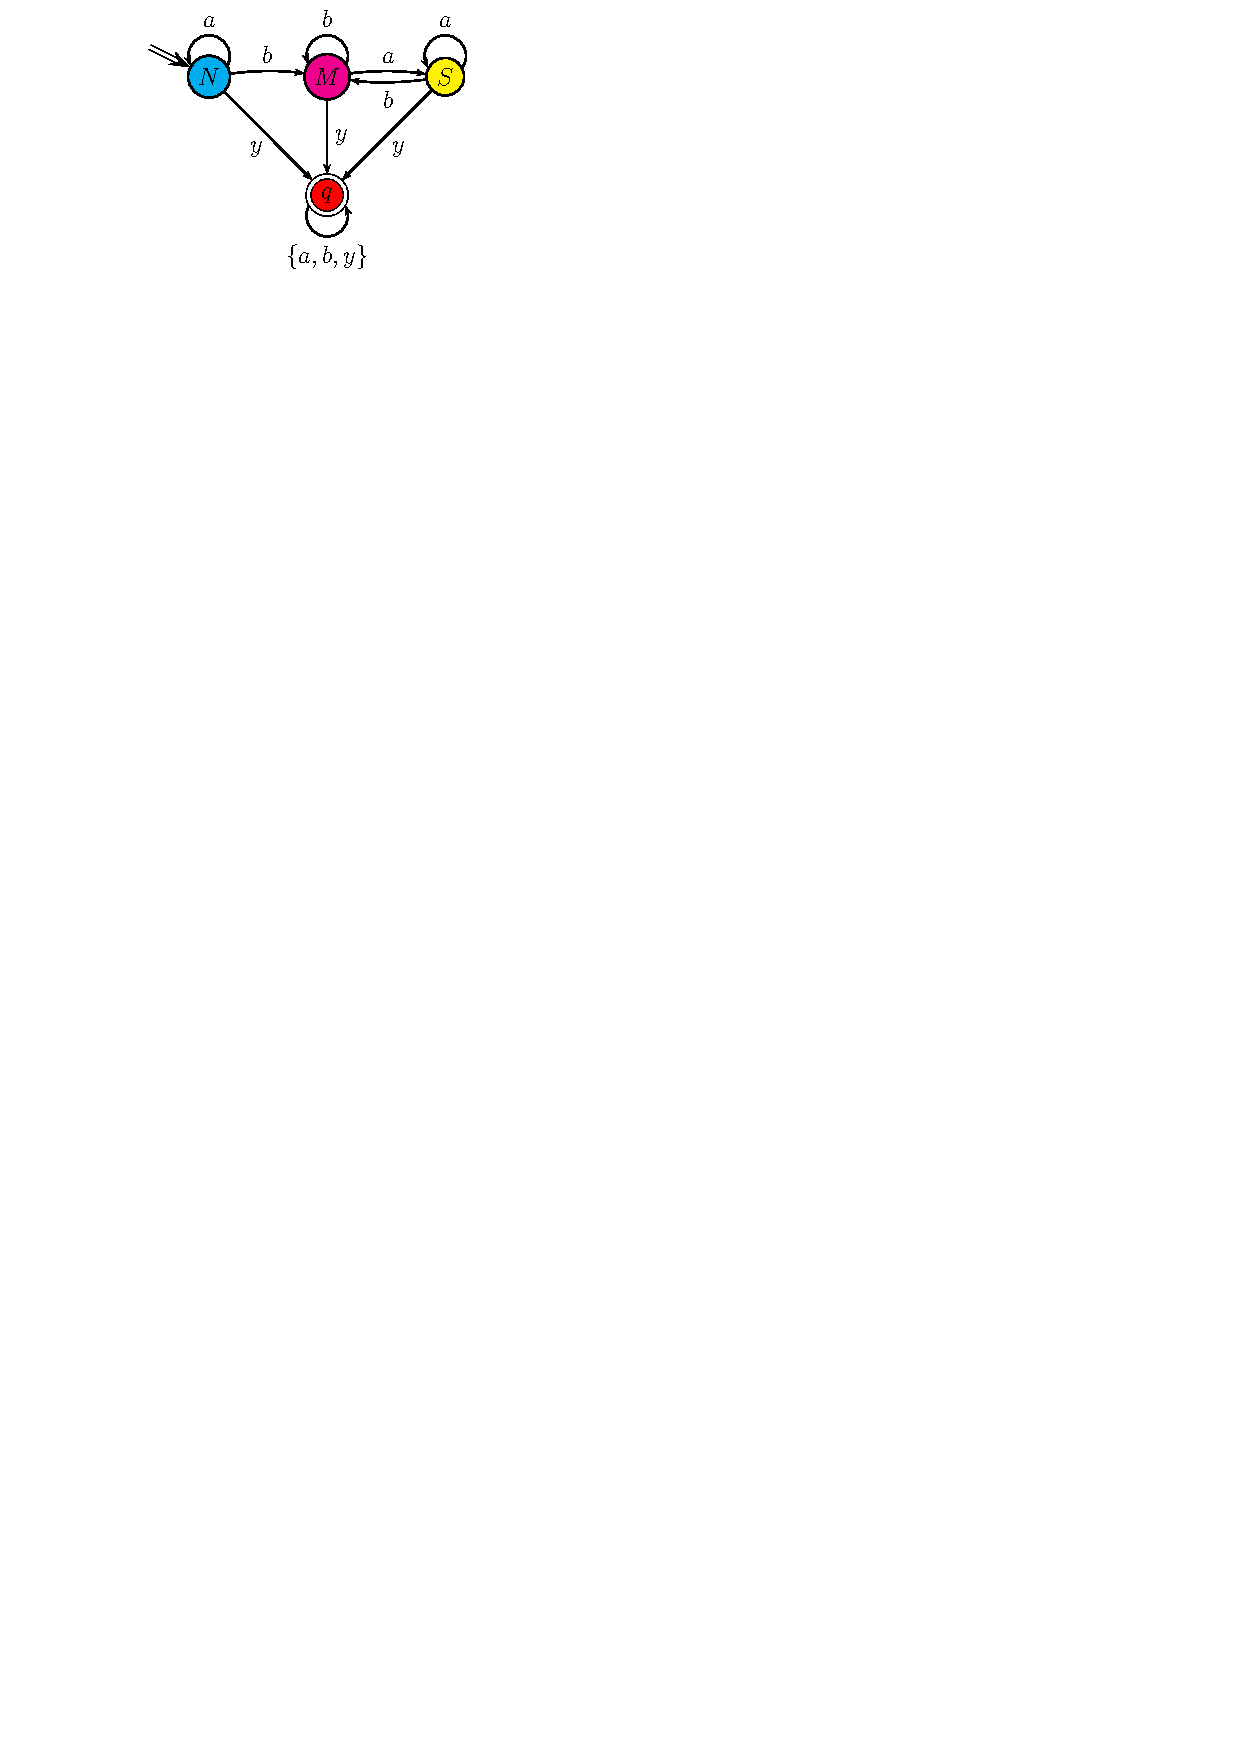
\includegraphics[bb=0 0 160 130]{images/pst.pdf}
\\ \kuti{\label{kuti:pstricks} \Y{PSTricks}による状態遷移図の描画} \\
{\small この状態遷移図を描くのに以下の入力をした.}\\
%「何かの状態遷移図に似てるよなぁ,あぁ TeX のあれかぁ」とかね.
\begin{InText}
%\usepackage[dvips]{graphicx,color}
%\usepackage{pst-all,pstcol}
\begin{TeXtoEPS}
\begin{math}
 \rput(0,3.5){\rnode{root}\relax}
 \cnodeput[fillstyle=solid,fillcolor=cyan](1,3){N}{N}
 \cnodeput[fillstyle=solid,fillcolor=magenta](3,3){M}{M}
 \cnodeput[fillstyle=solid,fillcolor=yellow](5,3){S}{S}
 \cnodeput[doubleline=true,fillstyle=solid,fillcolor=red](3,1){Q}{q}
 \psset{arrows=->,labelsep=3pt}
 \ncarc{N}{M}   \Aput{b}
 \ncarc{M}{S}   \Aput{a}
 \ncarc{S}{M}   \Aput{b}
 \ncline{N}{Q}  \Bput{y}
 \ncline{M}{Q}  \Aput{y}
 \ncline{S}{Q}  \Aput{y}
 \ncline[doubleline=true]{root}{N}
 \nccircle{->}{N}{10pt} \Bput{a}
 \nccircle{->}{M}{10pt} \Bput{b}
 \nccircle{->}{S}{10pt} \Bput{a}
 \nccircle[angleA=180]{->}{Q}{10pt} \Bput{\{a,b,y\}}
\end{math} 
\end{TeXtoEPS}
\end{InText}
\end{center}
\end{figure}
%
%
%
%\begin{figure}[htbp]
% \begin{center}
%
%\\ \kuti{明度と彩度の相関\label{kuti:meisai}}  \\
%{\small 明度とはどれだけ白に近いかという値で、
%黒の明度を0とし、白の明度を1として考えることが多い。
%彩度とは赤や青などの波長がどれだけ強いかを表す
%値で原色の赤の彩度を1とすると赤を含まない灰色の
%彩度は0になる。彩度を持たない色は無彩色と呼ばれている。}
% \end{center}
%\end{figure}

\makeatletter
\renewcommand{\theenumi}{\@arabic\c@enumi}
\makeatother



